\begin{frame}
    \frametitle{Git and GitHub}
    \framesubtitle{Getting started with Git}
    \addtocounter{nframe}{1}
    
	\begin{block}{Git command line environment}
		The command line is the only place you can run all Git commands.
    \end{block}

	\begin{block}{GUIs environment}
		GUIs implement only a partial subset of Git functionality for simplicity
    \end{block}
	

\end{frame}

\begin{frame}
	\frametitle{Git and GitHub}
    \framesubtitle{Getting started with Git}
    \addtocounter{nframe}{1}

	\begin{center}
		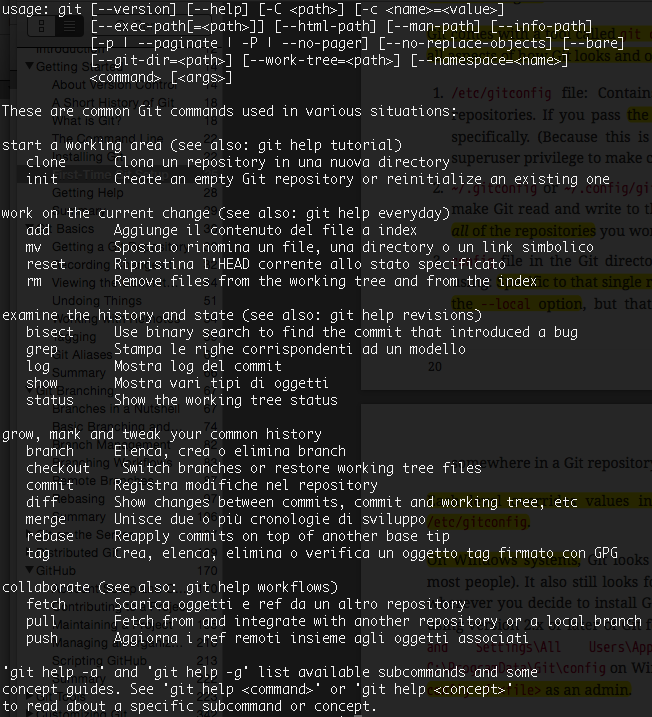
\includegraphics[width=.8\textwidth]{imgs/git-commands.png}
	\end{center}

\end{frame}

\begin{frame}
    \frametitle{Git and GitHub}
    \framesubtitle{Getting started with Git}
    \addtocounter{nframe}{1}
	
	\emph{Git comes with a tool called \textbf{git config} that lets you get and set configuration variables that control all aspects of how Git looks and operates}

	\begin{block}{git config}
		\begin{itemize}
			\item system (all users, all repositories)
			\item global (all repositories, single user)
			\item local (single repository, single user)
		\end{itemize}
    \end{block}

\end{frame}

\begin{frame}
    \frametitle{Git and GitHub}
    \framesubtitle{Getting started with Git}
    \addtocounter{nframe}{1}
	
	\emph{The first thing you should do when you install Git is to set your \textbf{user} name and \textbf{email} address
	}

	\begin{block}{git config}
		\begin{itemize}
			\item \texttt{git config --global user.name "Angelo Mario Del Grosso"}
			\item \texttt{git config --global user.email "angelo.delgrosso@ilc.cnr.it"}
		\end{itemize}
    \end{block}

\end{frame}

\begin{frame}
	\frametitle{Git and GitHub}
    \framesubtitle{Checking Your Settings}
    \addtocounter{nframe}{1}

	\begin{center}
		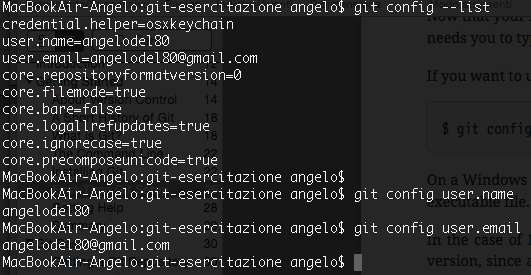
\includegraphics[width=.8\textwidth]{imgs/git-config.png}
	\end{center}

\end{frame}

\begin{frame}
    \frametitle{Git and GitHub}
    \framesubtitle{Getting started with Git}
    \addtocounter{nframe}{1}
	
	\begin{block}{help while using git}
		\begin{itemize}
			\item \texttt{git help <verb>}
			\item \texttt{man git-<verb>}
			\item \texttt{git <verb> --help}
			\item \texttt{git <verb> -h}
		\end{itemize}
    \end{block}

\end{frame}


\begin{frame}
    \frametitle{Git and GitHub}
    \framesubtitle{Getting started with Git}
    \addtocounter{nframe}{1}
	
	\begin{block}{fundamental capabilities}
		\begin{itemize}
			\item configure and initialize a repository
			\item tracking files
			\item stage and commit changes
			\item ignore certain files and file patterns
			\item undo mistakes
			\item browse the history
			\item view changes
			\item push and pull from remote repositories
		\end{itemize}
    \end{block}

\end{frame}

\begin{frame}
    \frametitle{Git and GitHub}
    \framesubtitle{Getting started with Git}
    \addtocounter{nframe}{1}
	
	\begin{block}{git repository}
		\begin{itemize}
			\item local directory that is not under version control, and turn it into a git repository
			\item clone an existing Git repository from elsewhere
		\end{itemize}
    \end{block}

\end{frame}

\begin{frame}
    \frametitle{Git and GitHub}
    \framesubtitle{Getting started with Git}
    \addtocounter{nframe}{1}
	
	\begin{block}{git repository init}
		\begin{itemize}
			\item \texttt{git init}
			\item \texttt{git clone <URL> <DIR>}
		\end{itemize}
    \end{block}

\end{frame}


\begin{frame}
    \frametitle{Git and GitHub}
    \framesubtitle{Getting started with Git}
    \addtocounter{nframe}{1}
	
	\begin{block}{git repository init}
		After \textbf{init} nothing in the project is tracked yet.\\
		Need to begin tracking those files and do an initial commit.
	\end{block}

	\begin{block}{specify the files you want to track}
		\begin{itemize}
			\item git add <FILE(S)>
			\item git commit -m "<MESSAGE>"
		\end{itemize}
	\end{block}
	
	\textit{Git repository with tracked files and an initial commit.}
    
\end{frame}


\begin{frame}
    \frametitle{Git and GitHub}
    \framesubtitle{Getting started with Git}
    \addtocounter{nframe}{1}
	
	\begin{block}{git clone repository}
		Every version of every file for the history of the project is pulled down by default when you run \texttt{git clone}
    \end{block}

\end{frame}

\begin{frame}
    \frametitle{Git and GitHub}
    \framesubtitle{Getting started with Git}
    \addtocounter{nframe}{1}
	
	\begin{block}{git repository init}
		Each file in your working directory can be in one of two states
	\end{block}

	\begin{block}{track files}
		\begin{itemize}
			\item tracked
			\item untracked
		\end{itemize}
	\end{block}
	
	\textit{Tracked files are files that were in the last snapshot; they can be \textbf{unmodified}, \textbf{modified}, or \textbf{staged}}
    
\end{frame}

\begin{frame}
	\frametitle{Git and GitHub}
    \framesubtitle{track files}
    \addtocounter{nframe}{1}

	\begin{center}
		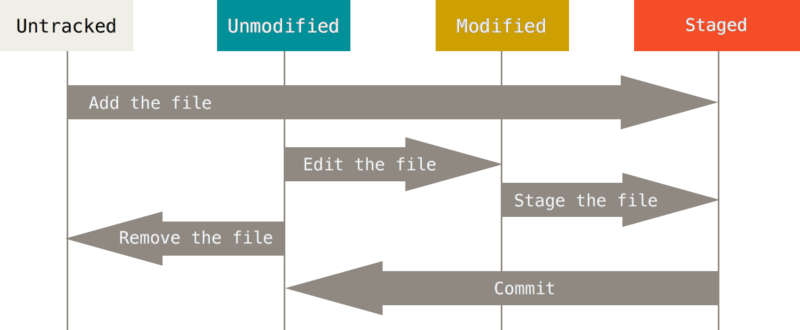
\includegraphics[width=.8\textwidth]{imgs/git-lifecycle-files.png}
	\end{center}

\end{frame}

\begin{frame}
	\frametitle{Git and GitHub}
    \framesubtitle{status files}
    \addtocounter{nframe}{1}

	\textit{To determine which files are in which state: \textbf{the git status command}}

	\begin{center}
		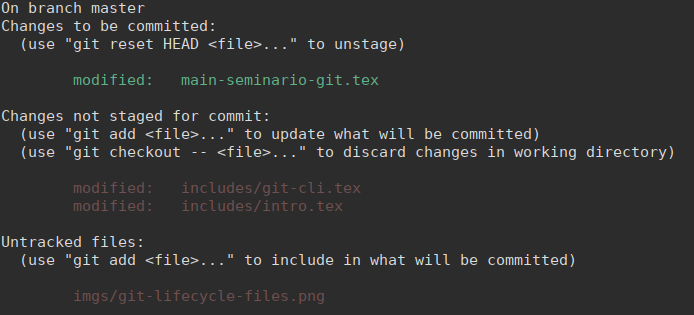
\includegraphics[width=.8\textwidth]{imgs/git-status.png}
	\end{center}

\end{frame}

\begin{frame}
	\frametitle{Git and GitHub}
    \framesubtitle{adding files}
    \addtocounter{nframe}{1}


	\begin{block}{git add}
		In order to begin tracking a new file, you use the \textbf{command git add}
	\end{block}

	\begin{block}{git add}
		file is now \textbf{tracked} and \textbf{staged} to be \textbf{committed}
	\end{block}

	\textit{The git add command \textbf{takes a path name} for either a file or a directory}
	

\end{frame}

\begin{frame}
	\frametitle{Git and GitHub}
    \framesubtitle{adding files}
    \addtocounter{nframe}{1}


	\begin{block}{git add}
		File that is tracked has been modified in the working directory but not yet staged
	\end{block}

	\begin{block}{git add}
		To stage a modified tracked file, you have to run the \textbf{git add command} again.
	\end{block}
	
	\textit{After git add, the files are staged and will go into your next commit}	

\end{frame}

\begin{frame}
	\frametitle{Git and GitHub}
    \framesubtitle{adding files}
    \addtocounter{nframe}{1}


	\begin{block}{git add}
		If you modify a file after you run git add, you have to run git add again to stage the latest version of the file
	\end{block}

	\begin{center}
		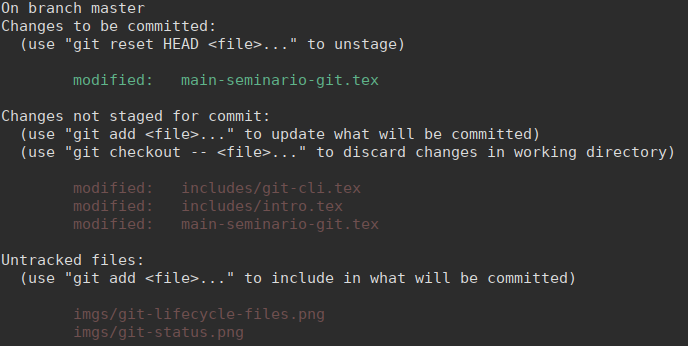
\includegraphics[width=.8\textwidth]{imgs/git-add-modify.png}
	\end{center}

\end{frame}

\begin{frame}
	\frametitle{Git and GitHub}
    \framesubtitle{ignoring files}
    \addtocounter{nframe}{1}


	\begin{block}{.gitignore file}
		If you’ll have a class of files that you don’t want to track
	\end{block}

	\begin{block}{.gitignore file}
		you can create a file listing patterns to match them named \textbf{.gitignore}.
	\end{block}

\end{frame}

\begin{frame}
	\frametitle{Git and GitHub}
    \framesubtitle{ignoring files}
    \addtocounter{nframe}{1}

	\begin{center}
		\texttt{more .gitignore}
	\end{center}
	
	\begin{center}
		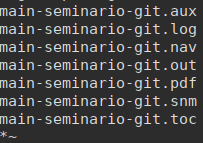
\includegraphics[width=.8\textwidth]{imgs/gitignore.png}
	\end{center}

\end{frame}

\begin{frame}
	\frametitle{Git and GitHub}
    \framesubtitle{viewing files}
    \addtocounter{nframe}{1}

	\begin{block}{git diff}
		know exactly what you changed, not just which files were changed\\
		by using the \textbf{git diff command}
	\end{block}

	\begin{block}{git diff}
		\begin{itemize}
			\item What have you changed but not yet staged (\texttt{git diff})
			\item what have you staged that you are about to commit (\texttt{git diff --staged})
		\end{itemize}
	
	\end{block}

\end{frame}

\begin{frame}
	\frametitle{Git and GitHub}
    \framesubtitle{viewing files}
    \addtocounter{nframe}{1}
	
	\begin{center}
		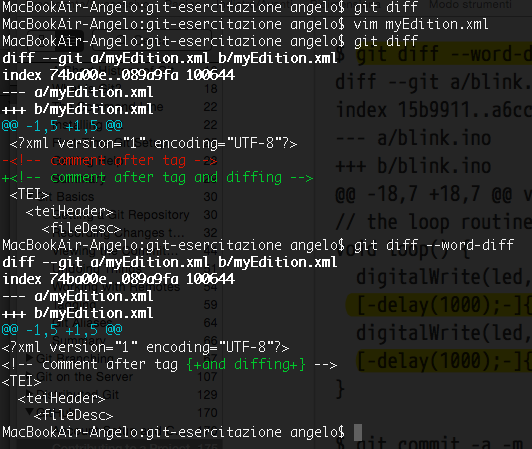
\includegraphics[width=.8\textwidth]{imgs/Diffing-line-word.png}
	\end{center}

\end{frame}

\begin{frame}
	\frametitle{Git and GitHub}
    \framesubtitle{committing files}
    \addtocounter{nframe}{1}

	\begin{block}{git commit}
		Any files you have created or modified that you haven’t run git add on since you edited them — won’t go into the commit.
	\end{block}

	\begin{block}{git commit}
		\begin{itemize}
			\item the simplest way to commit is to type (\texttt{git commit})
			\item type your commit message inline  (\texttt{git commit -m "message"})
		\end{itemize}
	
	\end{block}

\end{frame}

\begin{frame}
	\frametitle{Git and GitHub}
    \framesubtitle{committing files}
    \addtocounter{nframe}{1}

	\begin{block}{git commit}
		Every time you perform a commit, you’re recording a snapshot of your project that you can revert to or compare to later.
	\end{block}

	\begin{center}
		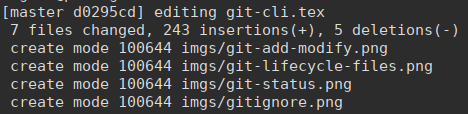
\includegraphics[width=.8\textwidth]{imgs/git-commit.png}
	\end{center}

\end{frame}

\begin{frame}
	\frametitle{Git and GitHub}
    \framesubtitle{removing files}
    \addtocounter{nframe}{1}

	\begin{block}{git rm}
		To remove a file from git, you have to remove it from your tracked files
	\end{block}

	\begin{block}{git rm}
		\begin{itemize}
			\item \texttt{git rm <FILE>}
			\item \texttt{git rm -f <FILE>}
			\item \texttt{git rm --cached <FILE>}
		\end{itemize}
	
	\end{block}

\end{frame}

\begin{frame}
	\frametitle{Git and GitHub}
    \framesubtitle{moving files}
    \addtocounter{nframe}{1}

	\begin{block}{git mv}
		If you rename a file in Git, no metadata is stored in Git that tells it you renamed the file
	\end{block}

	\begin{block}{git mv}
		\begin{itemize}
			\item \texttt{git mv <FILE_FROM> <FILE_TO>}
		\end{itemize}
	\end{block}

	\begin{block}{git mv}
		\begin{itemize}
			\item \texttt{mv <FILE_FROM> <FILE_TO>}
			\item \texttt{git rm <FILE_FROM>}
			\item \texttt{git add <FILE_TO>}
		\end{itemize}
	\end{block}
\end{frame}

\begin{frame}
	\frametitle{Git and GitHub}
    \framesubtitle{History of commits}
    \addtocounter{nframe}{1}

	\begin{block}{git log}
		\textbf{git log} lists the commits made in that repository in reverse chronological order, each commit with its checksum hash string, author’s name and email, date, the commit message.
	\end{block}

	\begin{block}{git log}
		\begin{itemize}
			\item \texttt{git log <options>}
		\end{itemize}
	\end{block}

\end{frame}

\begin{frame}
	\frametitle{Git and GitHub}
    \framesubtitle{History of commits}
    \addtocounter{nframe}{1}

	\begin{block}{git log}
		if you want to see some abbreviated stats for each commit, you can use \textbf{the --stat option}
	\end{block}

	\begin{block}{git log}
		\begin{itemize}
			\item \texttt{git log --stat}
		\end{itemize}
	\end{block}

\end{frame}

\begin{frame}
	\frametitle{Git and GitHub}
    \framesubtitle{History of commits}
    \addtocounter{nframe}{1}

	\begin{block}{git log --stat}
		\begin{center}
			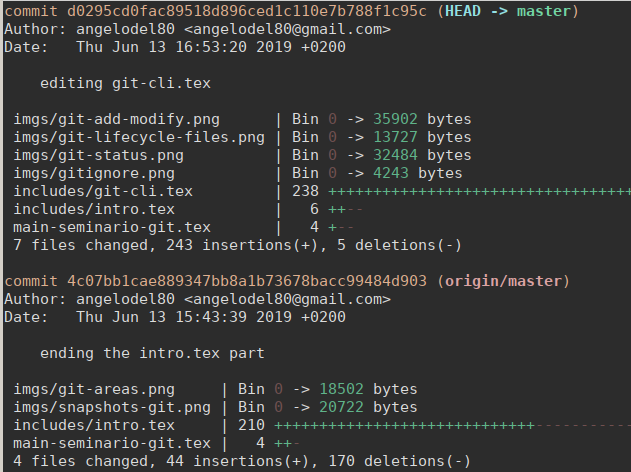
\includegraphics[width=.9\textwidth]{imgs/git-log-stats.png}
		\end{center}
	\end{block}

\end{frame}

\begin{frame}
	\frametitle{Git and GitHub}
    \framesubtitle{History of commits}
    \addtocounter{nframe}{1}

	\begin{block}{git log options}
		\begin{center}
			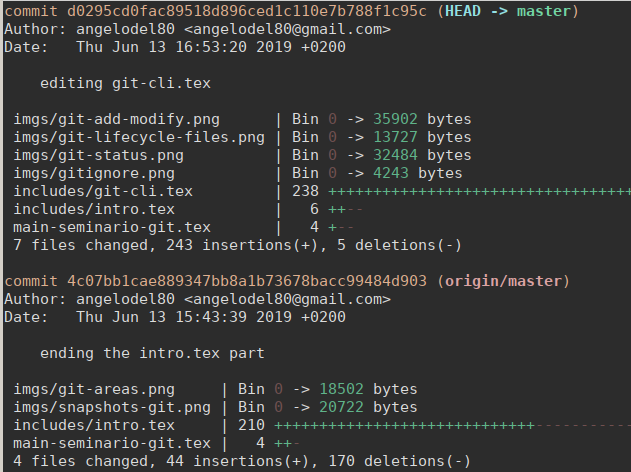
\includegraphics[width=.9\textwidth]{imgs/git-log-stats.png}
			%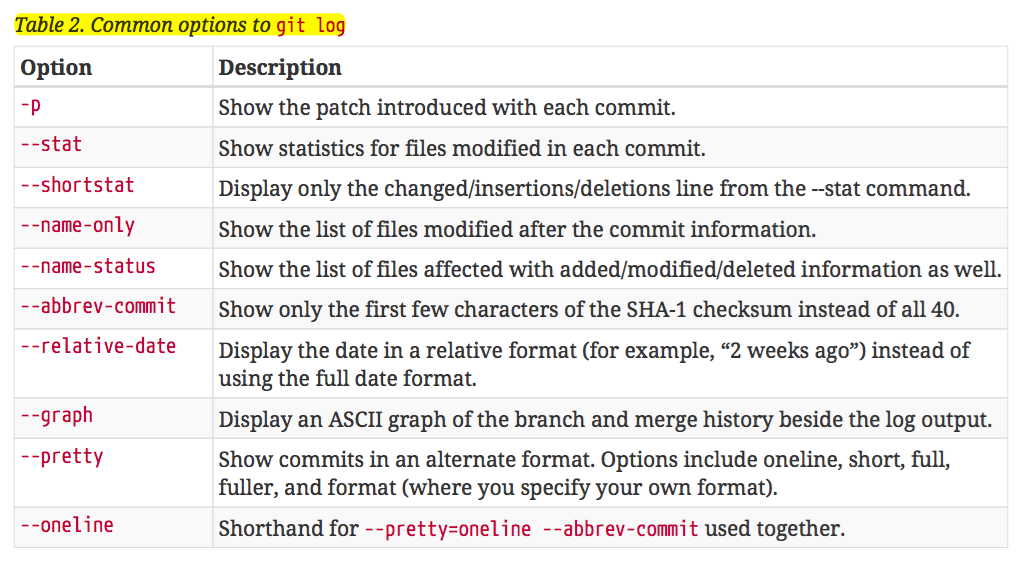
\includegraphics[width=.9\textwidth]{imgs/git-log-options.png}
		\end{center}
	\end{block}

\end{frame}

\begin{frame}
	\frametitle{Git and GitHub}
    \framesubtitle{History of commits}
    \addtocounter{nframe}{1}

	\begin{block}{git log --pretty}
		\begin{center}
			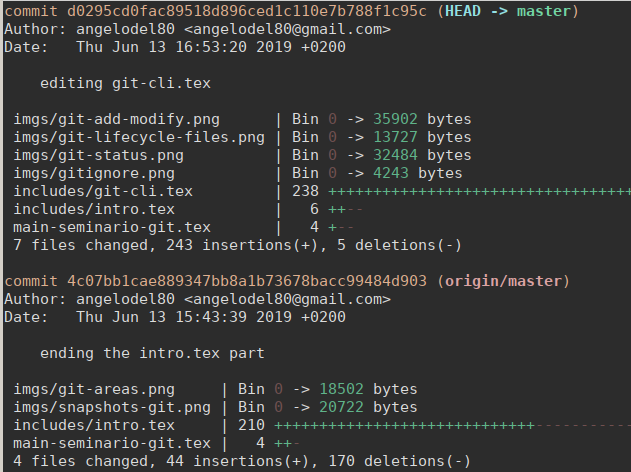
\includegraphics[width=.9\textwidth]{imgs/git-log-stats.png}
			%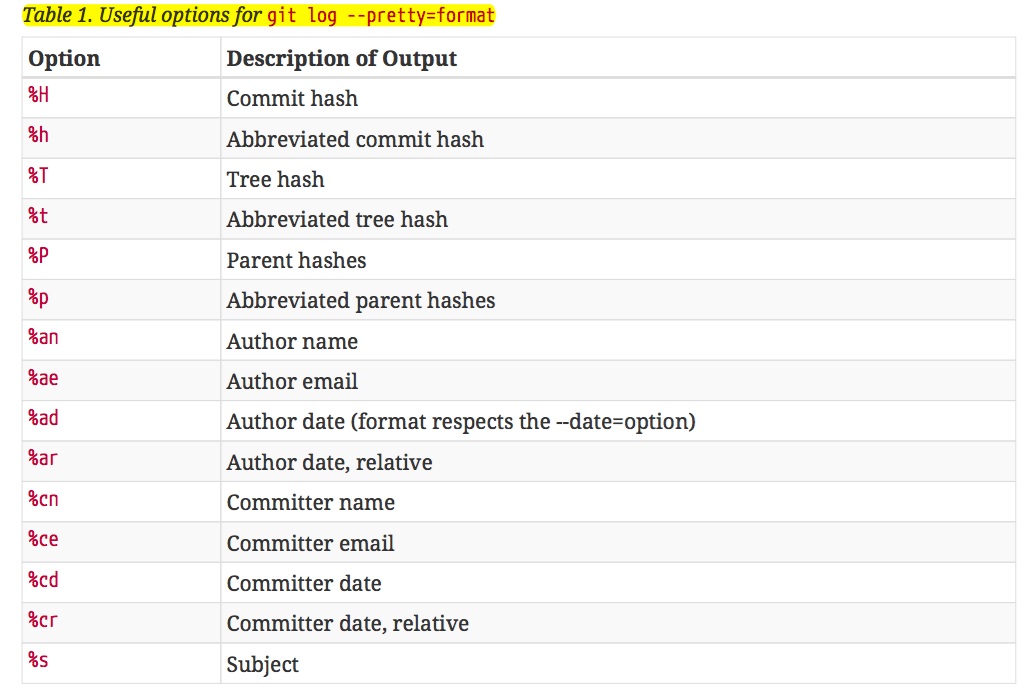
\includegraphics[width=.9\textwidth]{imgs/git-log-pretty.png}
		\end{center}
	\end{block}

\end{frame}

\begin{frame}
	\frametitle{Git and GitHub}
    \framesubtitle{History of commits}
    \addtocounter{nframe}{1}

	\begin{block}{git log limit options}
		\begin{center}
			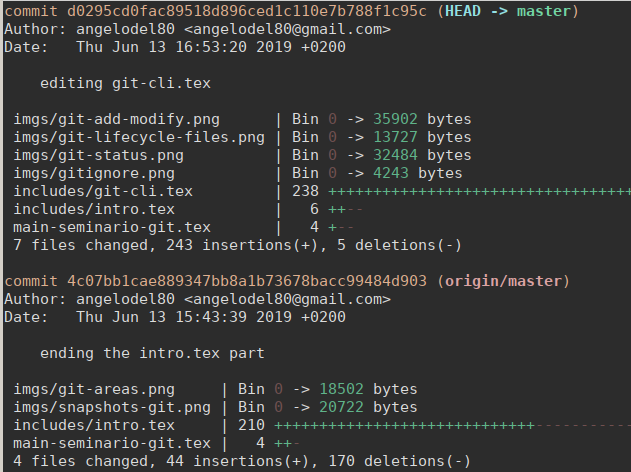
\includegraphics[width=.9\textwidth]{imgs/git-log-stats.png}
			%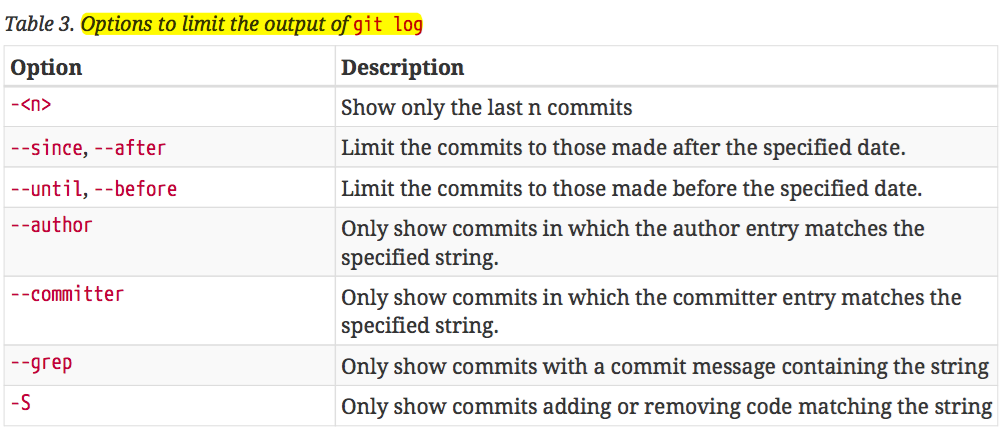
\includegraphics[width=.9\textwidth]{imgs/git-log-limits.png}
		\end{center}
	\end{block}

\end{frame}

\begin{frame}
	\frametitle{Git and GitHub}
    \framesubtitle{History of commits}
    \addtocounter{nframe}{1}

	\texttt{git log --pretty=``%h: %an -- %s'' --no-merges}
	\begin{block}{git log --pretty}
		\begin{center}
			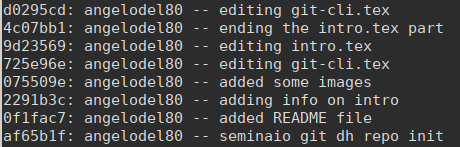
\includegraphics[width=.9\textwidth]{imgs/git-log-out.png}
		\end{center}
	\end{block}

\end{frame}



% frame 00
\begin{frame}
	\frametitle{Elementi di Codifica dei Caratteri}
	\framesubtitle{Definizioni}
	\addtocounter{nframe}{1}

	\begin{block}{Rappresentare il testo in formato digitale}
		L’adozione di metodologie informatiche per il trattamento dei testi richiede in primo luogo la disponibilità di un'adeguata rappresentazione dei dati testuali in formato digitale.
	\end{block}

\end{frame}

% frame 00b
\begin{frame}
	\frametitle{Elementi di Codifica dei Caratteri}
	\framesubtitle{Problemi di rappresentazione}
	\addtocounter{nframe}{1}

	\begin{center}
		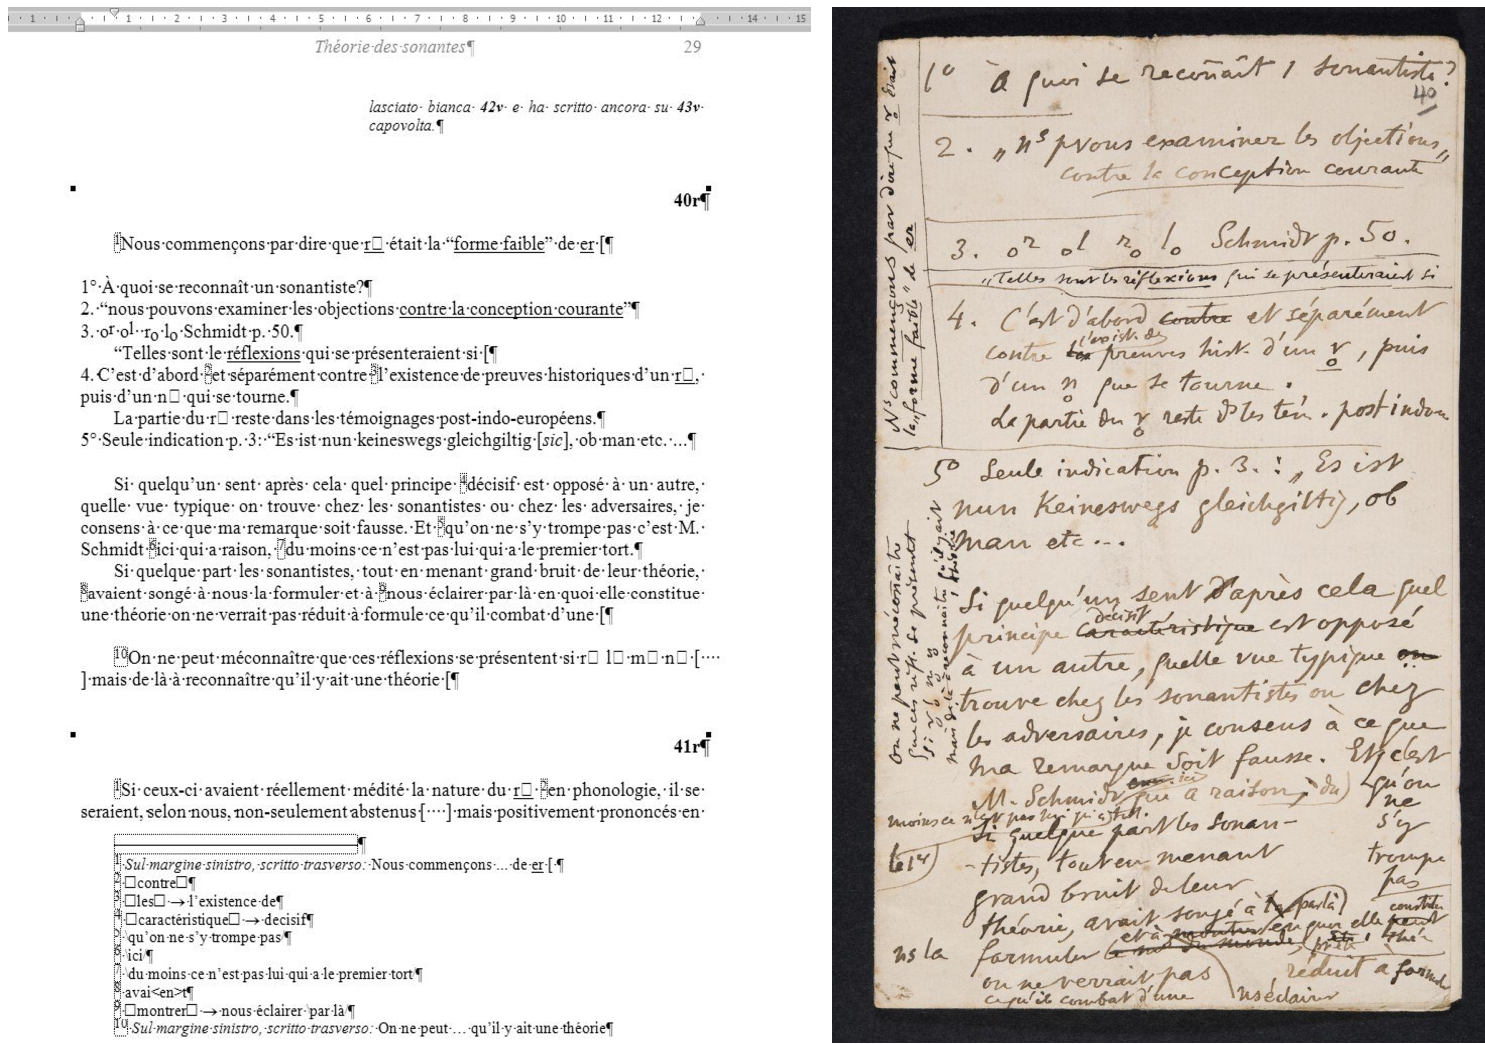
\includegraphics[width=.9\textwidth]{imgs/SaussureTrascrizione.pdf}
	\end{center}

\end{frame}


% frame 01
\begin{frame}
	\frametitle{Elementi di Codifica dei Caratteri}
	\framesubtitle{Definizioni}
	\addtocounter{nframe}{1}

	\begin{block}{Perché è importante la codifica dei caratteri}
		La codifica dei caratteri costituisce il grado zero (basso livello) della rappresentazione di testi su supporto digitale.
		\begin{center}
			\textit{Le codifiche dei caratteri sono la base di qualsiasi schema di codifica testuale}.
		\end{center}
	\end{block}

	\begin{block}{Rappresentazione digitale dei caratteri}
		I caratteri vengono rappresentati all’interno di un elaboratore mediante una sequenza di codici binari formati da opportune disposizioni di cifre composte da 0 e 1: 01100001 \textit{lettera a}
	\end{block}

\end{frame}



% frame 03
\begin{frame}
	\frametitle{Elementi di Codifica dei Caratteri}
	\framesubtitle{American Standard Code for Information Interchange}
	\addtocounter{nframe}{1}

	\begin{block}{Tabella Code Page ASCII 7 bit}
		%immagine di esempio Code Page ASCII (cp1252)
		\begin{center}
			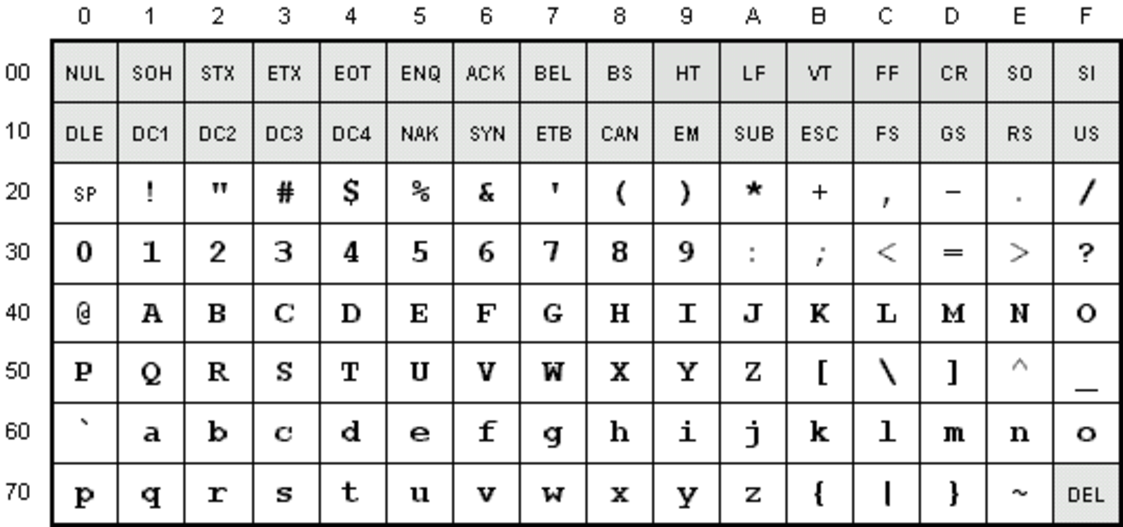
\includegraphics[width=.9\textwidth]{imgs/ascii-67.pdf}
		\end{center}

	\end{block}
	%\hline
	\begin{tiny}
		\begin{center}
			7 bit = 128 possibili caratteri; 32 caratteri di controllo; 96 caratteri effettivi
		\end{center}

	\end{tiny}

\end{frame}

% frame 0
\begin{frame}
	\frametitle{Elementi di Codifica dei Caratteri}
	\framesubtitle{Esempio codifica binaria}
	\addtocounter{nframe}{1}

	\begin{block}{codifica \textit{ciao mondo!} 7 bit ASCII}
		\begin{center}
			\textsc{6369 616f 206d 6f6e 646f 210a}
		\end{center}
	\end{block}

	\begin{block}{codifica \textit{ciao è mondo!} 8 bit ASCII}
		\begin{center}
			\textmd{6369 616f 20\textbf{e8} 206d 6f6e 646f 210a       }
		\end{center}
	\end{block}

	\begin{block}{codifica \textbf{ciao è mondo!} UNICODE UTF-8}
		\begin{center}
			6369 616f 20\textbf{c3 a8}20 6d6f 6e64 6f21 0a
		\end{center}
	\end{block}

\end{frame}

% frame 02
\begin{frame}
	\frametitle{Elementi di Codifica dei Caratteri}
	\framesubtitle{Definizioni}
	\addtocounter{nframe}{1}

	% \begin{block}{Character set, Code Set}
	%  - Character set
	%  - Code Set
	%  - Character encoding
	%  - Tabella del Code page
	% \end{block}

	\begin{description}
		\item [Character Set] Per le discipline che studiano i sistemi di scrittura e l'analisi del linguaggio naturale, un insieme di caratteri astratti è detto Character set (unità alfabetiche). Astratto perché non riguarda la rappresentazione materiale della forma sul supporto, ma è relativo alla forma mentale, fatta di simboli di codifica (referenti).
		\item [Coded Char Set] Per poter trattare un insieme di unità alfabetiche in formato digitale bisogna assegnare a ciascun carattere un numero intero non negativo detto code point.
		
	\end{description}

\end{frame}

% frame 02b
\begin{frame}
	\frametitle{Elementi di Codifica dei Caratteri}
	\framesubtitle{Definizioni}
	\addtocounter{nframe}{1}

	% \begin{block}{Character set, Code Set}
	%  - Character set
	%  - Code Set
	%  - Character encoding
	%  - Tabella del Code page
	% \end{block}

	\begin{description}
		\item [Character Encoding]  Il fine ultimo della codifica è quello di rappresentare una sequenza di caratteri in una sequenza di byte. La codifica di un carattere utilizza uno ``encoding schema'' che a sua volta mappa o trasforma ciascun code point in una sequenza di byte e quindi in ultima istanza in una sequenza di bit. 
		\item [Tabella del code page] Generalmente i code points sono espressi attraverso un sistema numerico esadecimale e disposti in una tabella di associazione.
	\end{description}

\end{frame}

% frame 02c
\begin{frame}
	\frametitle{Elementi di Codifica dei Caratteri}
	\framesubtitle{In sintesi}
	\addtocounter{nframe}{1}


	\begin{block}{Codifica dei caratteri}
		Quindi trasformare una sequenza di caratteri appartenenti ad un char set in una sequenza di byte (bit) significa prima di tutto trasformare/mappare ciascun carattere nel proprio corrispettivo code point e successivamente codificare/serializzare questo code point nella relativa sequenza di byte (bit).
	\end{block}

\end{frame}


% frame 0
\begin{frame}
	\frametitle{Elementi di Codifica dei Caratteri}
	\framesubtitle{Complessità e rappresentazione}
	\addtocounter{nframe}{1}

	\begin{block}{Complessità di rappresentazione universale dei caratteri}
		Se si considerano tutti i possibili alfabeti del mondo e le molteplici esigenze poste dalla scrittura delle fonti manoscritte antiche e medievali, ci si accorge che la realizzazione di un sistema universale per la codifica dei caratteri è un progetto molto complesso con svariate sfide da affrontare.
	\end{block}

\end{frame}

% frame 0
\begin{frame}
	\frametitle{Complessità della Codifica dei Caratteri}
	\framesubtitle{Un Esempio}
	\addtocounter{nframe}{1}

	\begin{center}
		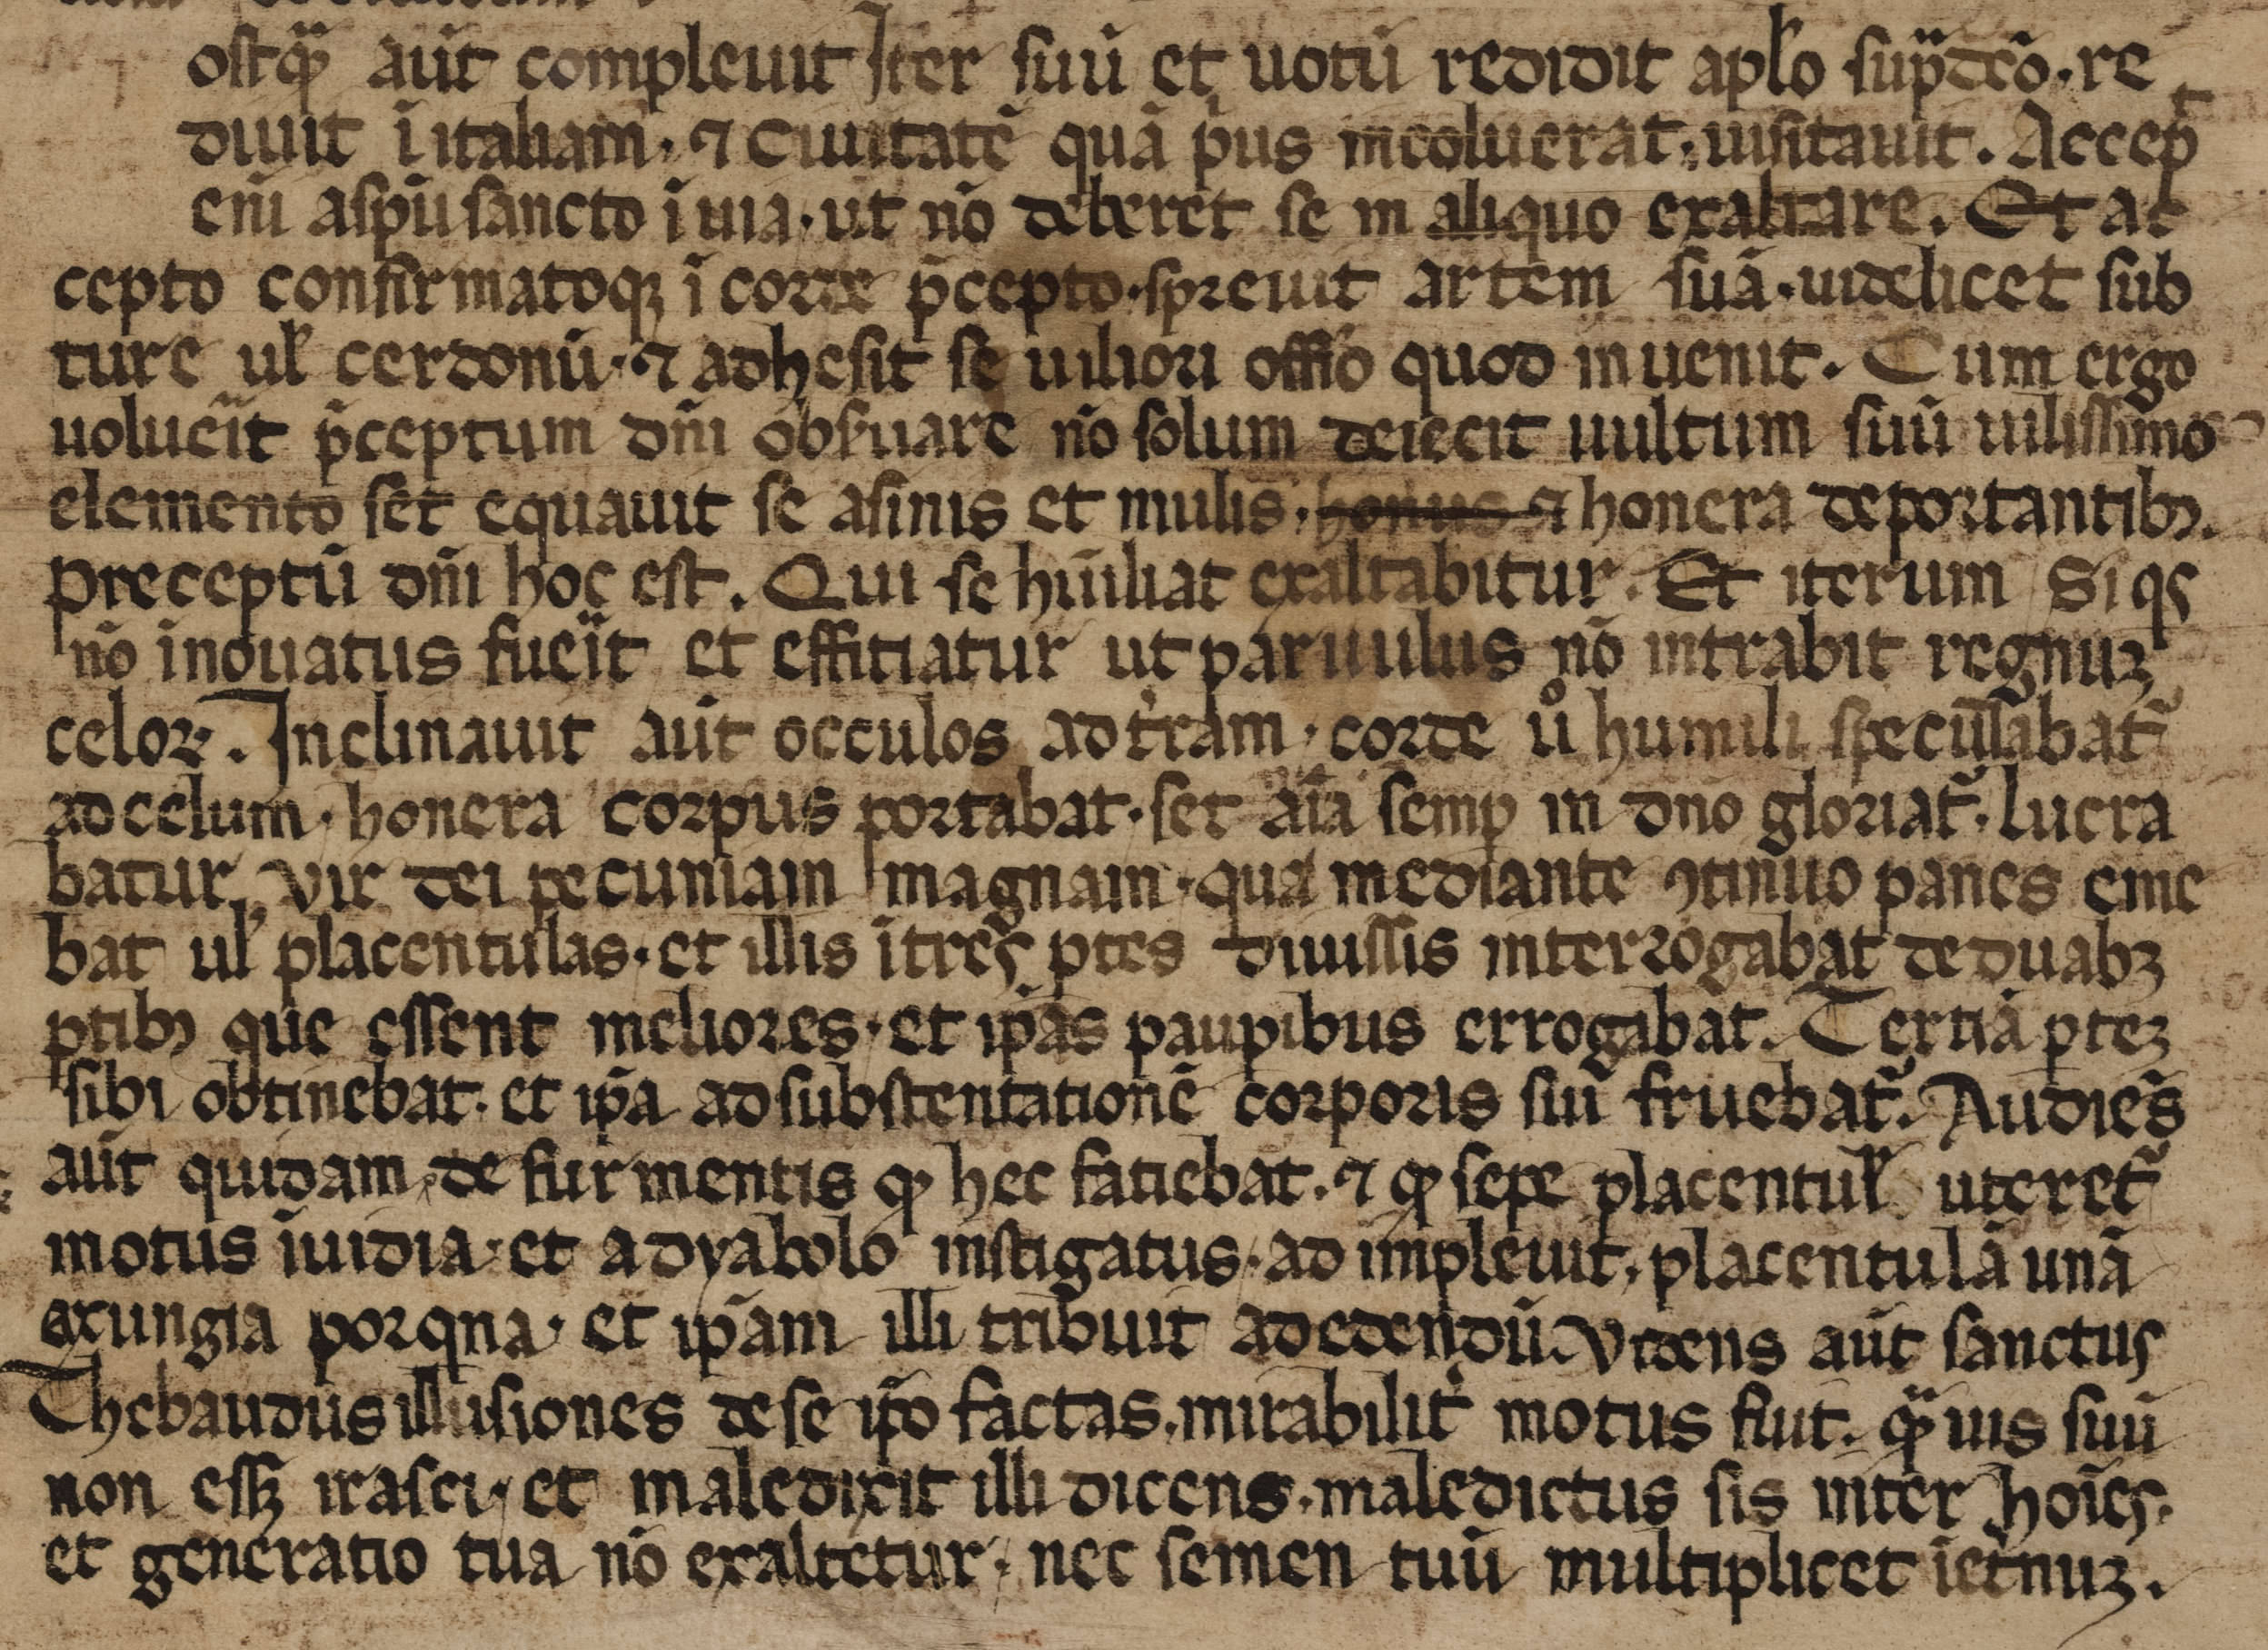
\includegraphics[width=.9\textwidth]{imgs/SnippetRotulo.jpg}
	\end{center}

\end{frame}

% frame 0
\begin{frame}
	\frametitle{Complessità della Codifica dei Caratteri}
	\framesubtitle{Un Esempio}
	\addtocounter{nframe}{1}

	\begin{center}
		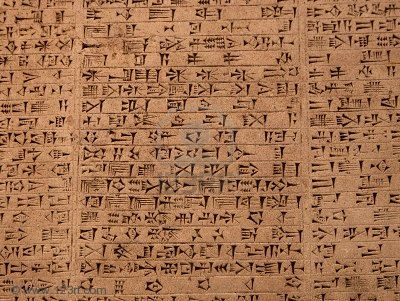
\includegraphics[width=.9\textwidth]{imgs/tavolettaArgilla.jpg}
	\end{center}

\end{frame}


\begin{frame}
	\frametitle{Elementi di Codifica dei Caratteri}
	\framesubtitle{Unicode}
	\addtocounter{nframe}{1}

	\begin{block}{Complessità di rappresentazione universale}
		Ad oggi, lo standard de facto per la codifica dei caratteri è lo UNICODE. Esso è in grado di codificare più di un milione di differenti unità alfabetiche, segni di interpunzione e diacritici, appartenenti a centinaia di diverse lingue.
	\end{block}

	\begin{block}{Complessità di rappresentazione universale}
		%(1.114.111)
		Unicode assegna i propri code point in un range che va da $0x0$ a $0x10FFFF$. In Unicode il code point viene  indicato con una ``U'' seguita da un segno ``+'' seguito a sua volta dall'esadecimale con padding del codice (es: U+0041 lettera A).
	\end{block}

\end{frame}

\begin{frame}
	\frametitle{Elementi di Codifica dei Caratteri}
	\framesubtitle{Unicode}
	\addtocounter{nframe}{1}

	\begin{block}{Unicode Transformation Format}
		Lo Unicode è un Coded Char Set e per essere concretamente serializzato su un supporto elettronico deve essere trasformato attraverso qualche tipo di schema di codifica.
		L'UTF (Unicode Transformation Format) mappa i code point Unicode in sequenze di byte (bit).
	\end{block}

	\begin{block}{UTF standards}
		Esistono tre tipi di schemi di codifica che vanno sotto il nome di UTF, ciascuno è identificato dal minimo numero di bit necessario a codificare ciascun code point: UTF-8; UTF-16; UTF-32. 
	\end{block}

\end{frame}

